\documentclass[10.5pt,compsoc,UTF8]{CjC}
\usepackage{ctex}
\usepackage{graphicx}
\usepackage{footmisc}
\usepackage{url}
\usepackage{multirow}
\usepackage{booktabs}
\usepackage{amsmath,amssymb}
\usepackage{xcolor,stfloats}
\usepackage{enumitem}
\usepackage{gbt7714}
\usepackage[hidelinks]{hyperref}
\newcommand{\upcite}[1]{\cite{#1}}

\setcounter{page}{1}
\graphicspath{{figures/}}
\xeCJKsetup{AutoFakeBold=true}
\tolerance=1600
\emergencystretch=1.5em
\hbadness=1500
\setlist{itemsep=1.5pt,topsep=2.5pt,parsep=0pt}
\setlength{\textfloatsep}{8pt plus 2pt minus 2pt}
\setlength{\dbltextfloatsep}{9pt plus 2pt minus 2pt}
\setlength{\intextsep}{8pt plus 2pt minus 2pt}
\setlength{\abovecaptionskip}{4pt}

% 页眉与页脚设置（与《计算机学报》模板一致）
\firstheadname{}
\firstfootname{}
\headevenname{\mbox{\quad}\hfill\mbox{\zihao{5-}{计\quad \quad 算\quad \quad 机\quad \quad 学\quad \quad 报}\hspace{45mm}\mbox{2026 年}}}
\headoddname{? 期 \hfill 朱梓涵：TA-MPPPB：面向虚存页表与多级预取的末级缓存替换策略}

\pagestyle{empty}

\begin{document}

\twocolumn[{
\vspace*{-20mm}
\noindent{\zihao{5-}%
\begin{tabular*}{\textwidth}{@{\extracolsep{\fill}}lcr@{}}
第?? 卷 第? 期 & 计\quad 算\quad \quad 机\quad \quad 学\quad \quad 报 & Vol. ?? No. ? \\
2026 年 11 月 & CHINESE JOURNAL OF COMPUTERS & Nov. 2026
\end{tabular*}}\\[0.2mm]
\rule{\textwidth}{0.6pt}\\[-2.2mm]\rule{\textwidth}{0.6pt}
\vspace{1mm}
\begin{center}
{\zihao{2}\heiti TA-MPPPB：面向虚存页表与多级预取的访存类型感知末级缓存替换策略}\\[0.15\baselineskip]
{\zihao{3}\fangsong 朱梓涵$^{1)}$}\\[0.05\baselineskip]
{\zihao{6}\songti $^{1)}$(中山大学广州东校区，广州 510006)}
\end{center}
\vspace{1mm}

{\noindent\zihao{5-}\heiti 摘\quad 要}\quad
{\zihao{5-}\songti
本文在支持五级页表游走（PTW）与多级硬件预取的现代 ChampSim 上严格复现多视角重用预测器 MPPPB（MICRO 2017），揭示其跨预取状态的显著“能力反转”：无预取时 MPPPB（Static MDPP）在 SPEC CPU2006（8 负载）与全量 28 负载分别较 LRU 提速 $+4.44\%$（优于 SHiP-PC 的 $+4.30\%$）与 $+4.49\%$；开启 \texttt{next\_line}+\texttt{ip\_stride} 后全 28 负载收益骤降至 $+1.34\%$（远逊 SHiP-PC 的 $+4.10\%$），开启 \texttt{spp\_dev} 更跌破 LRU 至 $-1.40\%$。解剖表明，\texttt{TRANSLATION}、\texttt{WRITE} 与 \texttt{PREFETCH} 以 $\mathrm{ip}=0$ 汇入 LLC，诱发 0 号桶踩踏、32 格历史环清零与页表误旁路（\texttt{spp\_dev} 下 PTW 命中率坠至 $23.07\%$）。本文提出零额外 SRAM 阵列、仅增 \textbf{20 bits（2.5 B）}寄存器的 \textbf{TA-MPPPB}，整合 Zero-PC 屏蔽、PTW 零旁路中游保护（$\mathrm{PLRU}=8$）、双模写回采样与需求缺失（\texttt{LOAD+RFO}）监督的正交双路集合决斗（\texttt{wsel\_}、\texttt{pfsel\_}）。覆盖 5 大数据集 28 负载的全满贯矩阵（336 场）与双预取器留一法消融（280 场，总计 616 场）证明：TA-MPPPB 在 \texttt{ip\_stride} 与 \texttt{spp\_dev} 下全 28 负载较 LRU 提速 \textbf{+5.91\%} 与 \textbf{+2.55\%}（超越 SHiP-PC $1.75\%/1.54\%$、MPPPB $4.51\%/4.00\%$），需求活跃子集（$\mathrm{LR\text{-}MPKI}\ge 2$）达 \textbf{+10.76\%} 与 \textbf{+4.99\%}，PTW 命中率升至 \textbf{69.38\%} 与 \textbf{55.14\%}。\par}\vspace{3pt}

{\noindent\zihao{5-}\heiti 关键词}\quad
{\zihao{5-}\songti 末级缓存替换；重用预测；虚存地址翻译；集合决斗；硬件预取；写回隔离}\\
{\noindent\zihao{5-}\heiti 中图法分类号}\quad {\zihao{5-} TP303} \qquad\qquad {\zihao{5-}\heiti DOI号：}{\zihao{5-}（课程研究报告）}\\[2pt]

\begin{center}
{\zihao{4}\bfseries TA-MPPPB: A Translation- and Access-Aware Multiperspective Last-Level Cache Replacement Policy}\\[0.12\baselineskip]
{\zihao{5} ZHU Zi-Han$^{1)}$}\\[0.04\baselineskip]
{\zihao{6} $^{1)}$(Guangzhou East Campus, Sun Yat-sen University, Guangzhou 510006)}
\end{center}
\vspace{1mm}

{\noindent\zihao{5-}\bfseries Abstract}\quad
{\zihao{5-}
Reproducing MPPPB (MICRO 2017, Static MDPP) on modern ChampSim with five-level page walks and multi-level prefetchers exposes a sharp prefetcher inversion: without prefetching, MPPPB beats LRU by $+4.44\%$ on SPEC CPU2006 (surpassing SHiP-PC's $+4.30\%$) and $+4.49\%$ across 28 traces; under \texttt{next\_line}+\texttt{ip\_stride}, it drops to $+1.34\%$ (trailing SHiP-PC's $+4.10\%$), and collapses to $-1.40\%$ under \texttt{spp\_dev}. Attribution traces this to zero-PC ($\mathrm{ip}=0$) \texttt{TRANSLATION}, \texttt{WRITE}, and \texttt{PREFETCH} requests aliasing Bucket~0, flushing the 32-entry PC ring, and falsely bypassing PTW lines. We propose \textbf{TA-MPPPB}, adding zero SRAM arrays and only \textbf{20 bits (2.5 B)} via Zero-PC shielding, non-bypass mid-tree PTW protection ($\mathrm{PLRU}=8$), dual-mode writeback sampling, and demand-miss-supervised orthogonal set dueling (\texttt{wsel\_}, \texttt{pfsel\_}). Across a full 28-workload $\times$ 3-regime $\times$ 4-policy matrix (336 runs) and dual-prefetcher LOO ablations (280 runs; 616 total), TA-MPPPB achieves \textbf{+5.91\%} (\texttt{ip\_stride}) and \textbf{+2.55\%} (\texttt{spp\_dev}) geomean IPC gains over LRU across all 28 traces—outperforming SHiP-PC by $1.75\%/1.54\%$ and MPPPB by $4.51\%/4.00\%$, reaching \textbf{+10.76\%} / \textbf{+4.99\%} on demand-intensive workloads and elevating PTW hit rates to \textbf{69.38\%} / \textbf{55.14\%}.\par}\vspace{3pt}

{\noindent\zihao{5-}\bfseries Keywords}\quad
{\zihao{5-} LLC replacement; reuse prediction; virtual translation; set dueling; prefetching; writeback isolation}
\vspace{4pt}
}]

\pagestyle{CjCheadings}
\thispagestyle{empty}
\footnotetext[0]{{\zihao{6}\songti 《并行计算机体系结构》课程期末研究论文（程序复现与原创微架构改进）。作者：朱梓涵，学号：24325356，E-mail: zhuzh67@mail2.sysu.edu.cn.}}

% 第一页仅保留中英文摘要栏。紧随其后的 \clearpage 使正文（第 1 节 引言）从第二页
% 页首以双栏开始，避免摘要栏几乎占满整页时引言标题与一两行正文被挤在页脚附近。
\clearpage
%======================================================================
\section{引\quad 言}
%======================================================================

随着现代乱序执行微处理器指令发射宽度与工作集规模持续扩张，主存（DRAM）访问延迟与片上计算速度之间的“存储墙”矛盾愈发突出。作为片上最后一道容量防线，末级缓存（Last-Level Cache, LLC）由于受到 L1 与 L2 缓存的高频过滤效应（Cache Filtering）影响，呈现低时间局部性与高“落地即死块”（Dead-on-Arrival）比例\upcite{jaleel2010rrip}，致使传统最近最少使用（LRU）替换策略因扫描冲刷与高硬件路数排序开销而在 LLC 层显著失效。

围绕 LLC 重用预测，体系结构领域发展出伪静态重引用间隔预测（RRIP/DRRIP\upcite{qureshi2007dip,jaleel2010rrip}）、指令签名命中预测（SHiP\upcite{wu2011ship}、SHiP++\upcite{young2017shippp}）及多视角感知机重用预测（MPPPB\upcite{jimenez2017mpppb}）等代表性算法。其中 Jiménez 等人于 MICRO 2017 提出的 MPPPB 融合 16 维哈希感知机特征表、$1/32$ 影子采样器（18 路真 LRU）与 15-bit 最小扰动树状伪 LRU（Static MDPP\upcite{teran2016mdpp}），在 ISCA 2017 第二届缓存替换锦标赛（CRC-2）及标准 SPEC CPU2006 基准上大幅领先传统方案\upcite{jimenez2017crc2}。

然而，当我们在包含完整五级虚拟内存页表游走（PTW）、非包容写回式缓存层级与多级硬件预取器的现代 ChampSim 平台\upcite{gober2022champsim}上完成 Static MDPP 底座的原版 MPPPB 复现后，将评测推向无预取与双硬件预取器全空间时，观测到一个尖锐的“能力反转（Inversion）”现象：在关闭硬件预取器时，原版 MPPPB 在 8 条 SPEC CPU2006 上相对 LRU 取得 $+4.44\%$ 几何平均 IPC 增益（压过经典 SHiP-PC 的 $+4.30\%$），在跨 5 个来源的 28 条综合负载上亦保持 $+4.49\%$ 的稳定收益；但一旦开启常规硬件预取（L1D \texttt{next\_line} + L2C \texttt{ip\_stride}），原版 MPPPB 跨 28 负载的收益陡降至 $+1.34\%$（远逊于 SHiP-PC 的 $+4.10\%$）；进一步切换至签名路径预取器 \texttt{spp\_dev}\upcite{kim2016spp} 后，MPPPB 的几何平均 IPC 全面跌破最基础的 LRU（\textbf{$-1.40\%$}，旧 SPEC06 子集更降至 $-2.19\%$，在 \texttt{450.soplex} 上倒退 $-7.03\%$）。

通过逐访问类型的底层跟踪与单变量受控归因，本文定位了该机制失效的根因：\textbf{现代处理器汇入 LLC 的四类核心流量（\texttt{LOAD/RFO}、\texttt{TRANSLATION}、\texttt{WRITE}、\texttt{PREFETCH}）在指令 PC 可见性与微架构停顿代价上存在剧烈割裂。}除核发出的阻塞型 \texttt{LOAD/RFO} 携带真实指令地址（$\mathrm{pc}\ne 0$）外，穿透 STLB 的五级页表游走（\texttt{TRANSLATION}）、L2 脏块驱逐回写（\texttt{WRITE}）及多级硬件预取（\texttt{PREFETCH}）在总线转发中统一以 $\mathrm{ip}=0$ 进入 LLC。原版 MPPPB 将全部请求塞入同一感知机预测—采样—旁路漏斗，诱发了四重并发病灶：（1）$\mathrm{ip}=0$ 流量在权重表 0 号桶发生剧烈别名踩踏；（2）32 格调用历史环 \texttt{pc\_ring} 被零值高频冲刷失忆；（3）决定虚实翻译链关键延迟的 \texttt{TRANSLATION} 块被误判真旁路（全 28 负载 \texttt{spp\_dev} 下页表命中率跌至 $23.07\%$，\texttt{429.mcf} 中更跌至 $0.83\%$）；（4）无阻塞后台 \texttt{WRITE} 与过量猜测预取污染采样器并挤占阻塞型需求工作集。

同期 ASPLOS 2025 研究\upcite{vavouliotis2025translation}同样指出了 PTW 缺失 PC 导致签名替换退化的问题，但其方案需跨 L1/L2/PTW 级联修改 MSHR 总线接口传递指令签名。与之对比，本文在\textbf{不修改任何缓存互连接口、且严格保持感知机与采样器 SRAM 阵列零扩容}（总状态由 $28.613\text{ KiB}$ 仅增 \textbf{20 bits} 至 $28.616\text{ KiB}$，远低于 CRC-2 的 $32\text{ KiB}$ 预算）的约束下，提出 \textbf{TA-MPPPB（Translation- \& Access-Aware MPPPB）}，做出如下四项主要贡献：

\begin{enumerate}
  \item \textbf{复现 Static MDPP 并量化预取器引发的 Zero-PC 耦合失效}：在修正偏移传递（\texttt{cache\_offset.patch}）的现代 ChampSim 上严格复现原版 MPPPB，通过 9 组单变量因果对照揭示“仅简单禁止预取旁路反而倒退至 $+1.48\%$”的非单调规律及写回命中的“采样饥饿（Write-Sampler Starvation）”效应。
  \item \textbf{提出零额外 SRAM 阵列的四通道解耦与双模决斗架构 TA-MPPPB}：实施 Zero-PC 特征与历史环屏蔽；为 \texttt{TRANSLATION} 设立零旁路、中游插入（$\mathrm{PLRU}=8$）与命中晋升硬保护；构建面向预取开关状态的双模 \texttt{WRITE} 采样协议；设计仅耗 20 bits 触发器的正交双路集合决斗器（\texttt{wsel\_}、\texttt{pfsel\_}），以核需求缺失（\texttt{LOAD+RFO}）作为唯一监督信号在 $\mathrm{PLRU}\in\{8,15\}$ 间在线仲裁。
  \item \textbf{完成 28 负载 $\times$ 3 预取状态 $\times$ 4 策略全满贯评测（336 场主对比）}：跨 SPEC CPU2006、SPEC CPU2017 Speed、GAP/XSBench、CVP-1 与 Qualcomm 服务器 5 大数据集冻结全部超参数评测，证明 TA-MPPPB 在无预取保持鲁棒、在 \texttt{ip\_stride} 与 \texttt{spp\_dev} 两大预取体系下均位居全策略第一，在阻塞需求活跃子集实现 $+10.76\%$ 与 $+4.99\%$ 加速，在 \texttt{spp\_dev} 高压力子集对原版 MPPPB 实现 $15/0/0$ 全胜。
  \item \textbf{完成全 28 负载 $\times$ 双预取器留一法（LOO）消融（280 场）与边界剖析}：覆盖全部 28 条负载的 \texttt{ip\_stride} 与 \texttt{spp\_dev} 五重正交消融证明了预取仲裁（最高挽回 $+15.85\%$）、写回仲裁与固定中游 PTW 保护的不可或缺性，定量揭示动态页表决斗在跨未见负载上导致 PTW 命中率崩塌至 $12.88\%\sim 15.78\%$ 的失稳机理，并实证解剖了 \texttt{effective\_\allowbreak ip} 与 MSHR 合并机制耦合的 $<0.23\%$ 微扰边界。
\end{enumerate}

%======================================================================
\section{相关工作}
%======================================================================

\subsection{启发式与最小扰动硬件替换策略}

为克服真 LRU 在高路数缓存中的排序硬件开销与扫描退化问题，Qureshi 等人\upcite{qureshi2007dip}提出动态插入策略 DIP，首创借助 64 个领跑集合与 10-bit 饱和计数器在 LRU 与低频 BIP 间自适应切换的集合决斗（Set-Dueling）范式。Jaleel 等人\upcite{jaleel2010rrip}进一步提出 RRIP 家族（SRRIP/DRRIP），为每行维护 2-bit 重引用预测值，有效抵御长流扫描冲刷。在此基础上，Teran 等人\upcite{teran2016mdpp}提出最小扰动放置与提升（MDPP），使用每组 15-bit 树状伪 LRU（Tree-PLRU）精细表征 16 路有序度，允许新行按死块置信度插入不同树深（如 $\mathrm{PLRU}\in\{0,12,15\}$）或直接触发不占槽位的真旁路（True Bypass），并在命中时采用局部微步向量 \texttt{kVecMdpp} 仅上移一级以保护其余驻留热行。

\subsection{签名预测、多视角感知机与重用学习}

基于同指令地址（PC）具有相似重用特征的局部性规律，Wu 等人\upcite{wu2011ship}提出 SHiP，采用 16K 项 3-bit 饱和计数器（SHCT）在线学习 PC 重用信用；Young 等人\upcite{young2017shippp}在 SHiP++ 中进一步针对预取与写回修正了特征更新策略。为超越单 PC 视角，Teran 等人\upcite{teran2016perceptron}与 Jiménez 等人\upcite{jimenez2017mpppb}提出基于 16 维哈希特征表的多视角感知机重用预测架构 MPPPB，协同 1/32 影子采样器（18 路真 LRU）与死区强化训练同时指导旁路、多级插入与提升决策，成为 CRC-2 竞赛标杆算法\upcite{jimenez2017crc2}。另一方面，Hawkeye\upcite{jain2016hawkeye}与 Glider\upcite{shi2019glider}借助在线 Belady 最优替换（OPTgen）或深度序列模型监督预测重用；但现有学习型策略多隐含假定 LLC 访问具备完整 PC 语义，缺乏对现代多级虚存与回写混合流量的内生隔离。

\subsection{页表、写回与预取感知的缓存协同管理}

围绕现代复杂层次结构下的异构 LLC 流量管理，近期顶会研究从三个维度切入：（1）\textbf{页表翻译保护}：Vavouliotis 等人\upcite{vavouliotis2025translation}（ASPLOS 2025）指出多级页表游走穿透 STLB 到达 LLC 后因缺失指令 PC 而恶化替换性能，采用修改跨层 MSHR 总线携带触发指令签名的方式加以解决；（2）\textbf{写回流量管理}：CARE\upcite{lu2023care}强调脏写回属于非阻塞后台写请求、应让位于需求读，而早期写回研究亦发现部分程序存在热写回重读现象；（3）\textbf{预取感知替换}：PACMan\upcite{wu2011pacman}与 Harmony\upcite{jain2018harmony}证明预取器开启时应聚焦最小化阻塞核心需求缺失而非无差别总缺失。本文 TA-MPPPB 首次在不修改任何片上总线接口与不增加 SRAM 阵列的严格硬件预算内，将上述三类流量的差异化治理闭环统一于 20 bits 正交控制机制。

%======================================================================
\section{基线复现与预取反转机理归因}
%======================================================================

\subsection{从 Static MDPP 严格复现到预取“能力反转”}

我们在 ChampSim 官方现代主干（\texttt{develop@\allowbreak 410cee62d9}）上发现：向替换模块传入物理地址时默认清零块内低 6 位偏移，导致依赖行内字节偏移的 \texttt{offset} 视角特征失效。为此，我们在模拟器接口层应用了仅 2 行的 \texttt{cache\_\allowbreak offset.patch}，使 \texttt{find\_\allowbreak victim}、\texttt{replacement\_\allowbreak cache\_\allowbreak fill} 与 \texttt{update\_\allowbreak replacement\_\allowbreak state} 统一接收完整未对齐字节地址（经核查对 LRU 与 SHiP-PC 行为零影响）。

在此公平底座上，我们严格遵循作者 CRC-2 单核 Static MDPP 规范复现了原版 \texttt{MPPPB}（15-bit Tree-PLRU + \texttt{kVecMdpp} 微步提升 + 返回 \texttt{way=16} 真旁路 + 死区强化训练，无预取与有预取分别采用原文 Table 1/2 配置参数）。如图~\ref{fig:repro_attr}(a) 所示，在 8 条 SPEC CPU2006 经典负载（50M 预热 + 150M 仿真）上呈现出急剧的跨预取器能力反转：
\begin{itemize}
  \item \textbf{无预取（No-Prefetch）}：原版 \texttt{MPPPB} 相对 LRU 取得 \textbf{+4.44\%} 几何平均 IPC 提升，稳定压过经典基线 \texttt{SHiP-PC}（\textbf{+4.30\%}），成功复现 MICRO 2017 原文结论。
  \item \textbf{常规预取（\texttt{next\_line}+\texttt{ip\_stride}）}：原版 \texttt{MPPPB} 收益骤降至 \textbf{+1.66\%}，不仅被 \texttt{SHiP-PC}（\textbf{+2.56\%}）明显反超，更在 \texttt{437.leslie3d} 与 \texttt{470.lbm} 上退化至 $-2.46\%$ 与 $-1.46\%$。
  \item \textbf{强路径预取（\texttt{next\_line}+\texttt{spp\_dev}）}：原版 \texttt{MPPPB} 进一步崩溃至 \textbf{-2.19\%}（全面劣于 LRU），在 \texttt{450.soplex} 与 \texttt{429.mcf} 上暴跌 $-7.03\%$ 与 $-5.86\%$，而页表 \texttt{TRANSLATION} 命中率跌至仅 \textbf{4.50\%}。
\end{itemize}

\begin{figure*}[t]
  \centering
  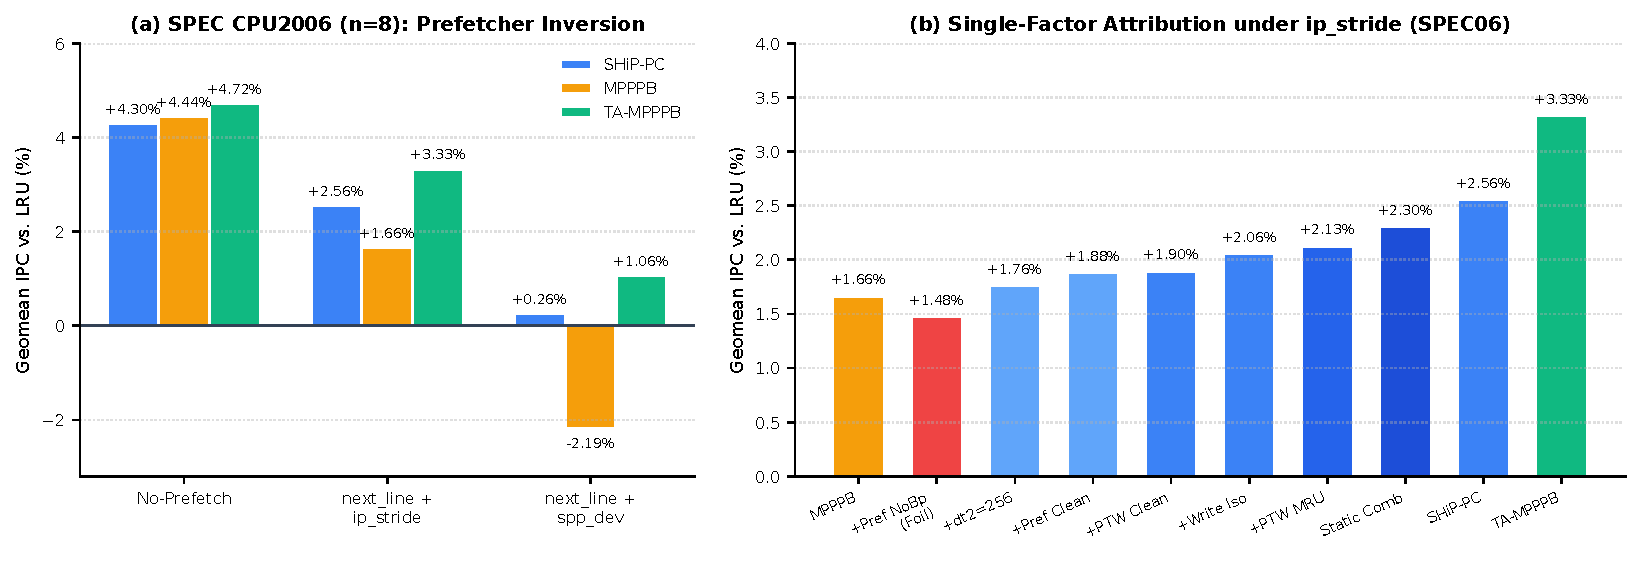
\includegraphics[width=0.96\textwidth]{fig2_repro_attr.pdf}
  \caption{基线复现验证与开启预取后的单变量因果归因（SPEC CPU2006，$n=8$）：(a) 从无预取至双硬件预取器切换引发的原版 MPPPB“能力反转”；(b) \texttt{next\_line}+\texttt{ip\_stride} 下从原版 MPPPB（$+1.66\%$）到 TA-MPPPB（$+3.33\%$）的单变量受控归因链。}
  \label{fig:repro_attr}
\end{figure*}

\subsection{Zero-PC 混合流量的四重并发失效机理}

解剖 ChampSim \texttt{src/cache.cc} 报文链路可见：\texttt{LOAD} 与 \texttt{RFO} 携带精确触发指令地址（$\mathrm{pc}\ne 0$），而 \texttt{next\_line} / \texttt{ip\_stride} / \texttt{spp\_dev} 产生的 \texttt{PREFETCH}、五级页表游走 \texttt{TRANSLATION} 以及 L2 脏写回 \texttt{WRITE} 在跨层级转发时均以 $\mathrm{ip}=0$ 到达 LLC。原版 MPPPB 将上述五类语义迥异的访问不加区分地注入同一感知机预测与采样漏斗，直接诱发了四重耦合失效（图~\ref{fig:arch}(a)）：

\begin{enumerate}
  \item \textbf{权重表 0 号桶高强度踩踏}：原版有预取特征集中多达 9 维直接索引或异或当前 $\mathrm{ip}$。海量 $\mathrm{ip}=0$ 请求同步坍缩至权重槽 $\mathrm{Table}[f][0]$，使预取、写回与页表信用在一个 6-bit 有符号槽位上高频互覆。
  \item \textbf{32 格调用历史环失忆（\texttt{pc\_ring} Flushing）}：原版每逢 LLC 访问便无条件写入 \texttt{pc\_ring[stamps \% 32]}。高密度到达的写回、预取与页表请求瞬间将 32 格历史缓冲冲刷为全 0，导致 $w=2,4$ 等历史路径视角特征实质失效。
  \item \textbf{高延迟页表行遭误旁路}：0 号桶正权重漂移一旦触发真旁路（$\mathrm{way}=16$），每一次 STLB 未命中都将被迫重走五级主存页表游走。\texttt{ip\_stride} 下旧 8 条负载中 MPPPB 累计误旁路重要预取 908.8 万次；新 20 条上误旁路 \texttt{PREFETCH} 高达 3{,}835.5 万次、\texttt{TRANSLATION} 高达 93.6 万次（表~\ref{tab:probe_stats}），导致 \texttt{429.mcf} 的 \texttt{TRANSLATION} 命中率被压低至 \textbf{0.23\%}（\texttt{470.lbm} 更低至 \textbf{0.00\%}）。
  \item \textbf{写回与预取挤占采样器及需求席位}：以 \texttt{429.mcf} 和 \texttt{450.soplex} 为例，L2 写回高达数十万次，且高达 $91\%\sim 99.9\%$ 命中早先由需求读建立的采样条目；与此同时大量猜测性预取扰动采样分布并挤占关键需求数据块。
\end{enumerate}

\begin{figure*}[t]
  \centering
  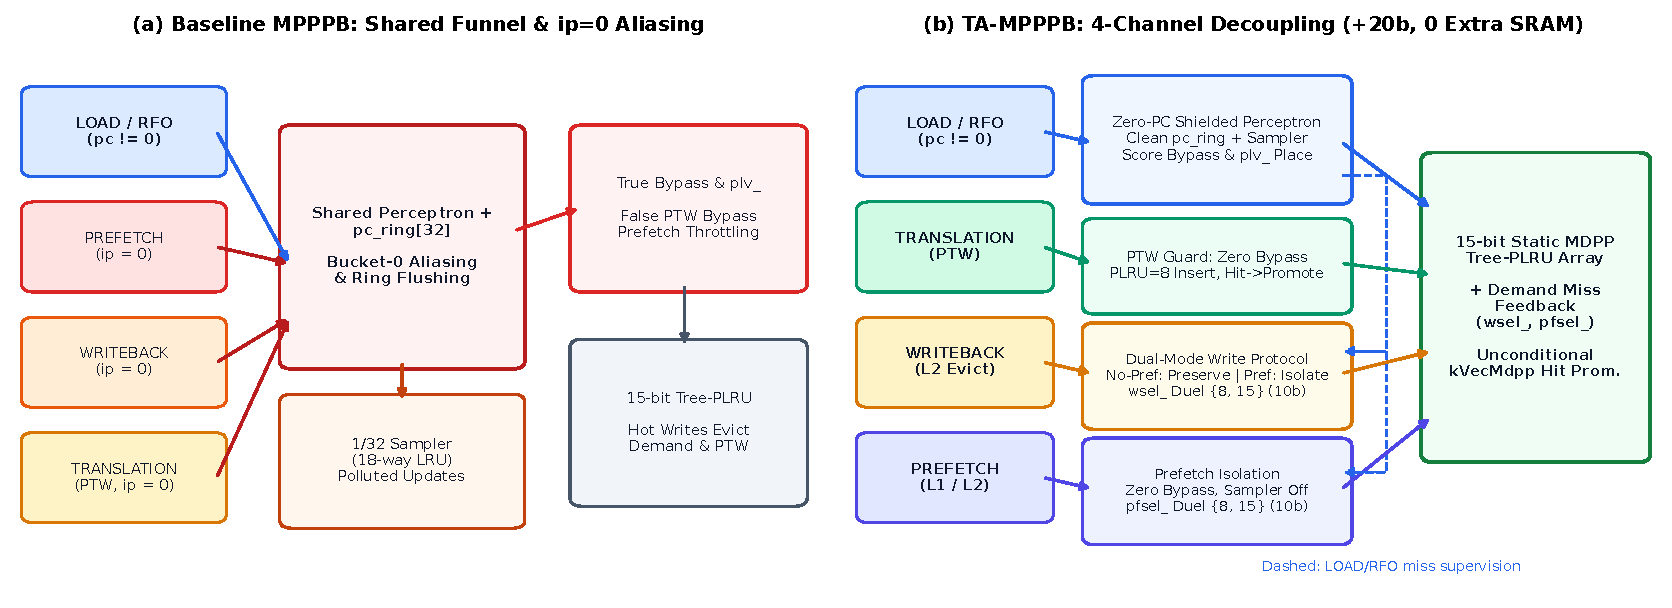
\includegraphics[width=0.98\textwidth]{fig1_arch.pdf}
  \caption{架构机理对比：(a) 原版 MPPPB 将全部请求汇入共享漏斗，导致 0 号桶踩踏、\texttt{pc\_ring} 清零与页表误旁路；(b) TA-MPPPB 实施四通道访存语义解耦、Zero-PC 特征屏蔽及需求缺失监督的正交双路集合决斗（虚线表示 \texttt{LOAD/RFO} 缺失监督信号）。}
  \label{fig:arch}
\end{figure*}

\subsection{前向单变量受控归因链}

为精确剥离各失效因素的独立影响，我们在 \texttt{ip\_stride} 下的原版 \texttt{MPPPB}（$+1.66\%$）上逐项构造受控单变量变体，结果如图~\ref{fig:repro_attr}(b) 所示：
\begin{itemize}
  \item \textbf{阈值放宽与零 PC 解耦}：将旁路决斗上限 $\mathrm{dt}_2$ 从 48 放宽至 256（\texttt{+dt2=256}）提升至 $+1.76\%$；仅净化零 PC 预取（\texttt{+Pref Clean}）与零 PC 页表（\texttt{+PTW Clean}）分别升至 $+1.88\%$ 与 $+1.90\%$，证实清除 0 号桶与历史环污染具有独立正收益。
  \item \textbf{单域保护与静态隔离}：仅禁止写回污染采样并放宽写回淘汰（\texttt{+Write Iso}）升至 $+2.06\%$（在 \texttt{429.mcf} 与 \texttt{470.lbm} 均获显著增益，却使存在写回重用的 \texttt{450.soplex} 回退 $-1.78\%$）；仅禁止页表旁路并保护至 MRU（\texttt{+PTW MRU}）提升至 $+2.13\%$。
  \item \textbf{关键负向对照（\texttt{+Pref NoBp}）}：如果仅简单禁止 \texttt{PREFETCH} 旁路而不配套分级驻留仲裁，IPC 反而从 $+1.66\%$ 跌落至 \textbf{+1.48\%}（全隔离 \texttt{p1\_pref\_iso} 更跌至 \textbf{+1.44\%}），原因在于大量低精度无用预取强行滞留 LLC 并挤出热需求行。
  \item \textbf{静态正交组合极限}：将上述静态规则简单叠加（\texttt{Static Comb}）达到 $+2.30\%$，依然落后于 \texttt{SHiP-PC}（$+2.56\%$）。这一归因结果直接揭示了突破路径：\textbf{必须对 \texttt{WRITE} 与 \texttt{PREFETCH} 的缓存占位深度建立基于核需求代价的在线动态自适应仲裁。}
\end{itemize}

%======================================================================
\section{TA-MPPPB 架构设计与硬件预算}
%======================================================================

基于第 3 节的机理诊断，本文提出 \textbf{TA-MPPPB}（图~\ref{fig:arch}(b)），在保留 16 维感知机、$1/32$ 影子采样器与 15-bit Tree-PLRU 主干的基础上，对进入 LLC 的四类访存请求实施精确分流与零增量 SRAM 仲裁。

\subsection{Zero-PC 特征屏蔽与历史环净化}

对于进入主感知机 \texttt{predict()} 的请求，TA-MPPPB 检查每条特征是否涉及当前指令 PC（$w=0$ 或含 \texttt{mix\_pc} 异或开关）。当且仅当开启屏蔽（\texttt{ab\_mask\_zero\_pc\_=true}）且有效指令地址 $\mathrm{eff\_ip}=0$ 时，直接将对应特征索引置零并跳过权重表累加，杜绝 $\mathrm{ip}=0$ 请求借由 0 号权重槽误导旁路打分。在 \texttt{pc\_ring[32]} 历史环入口处，严格过滤所有 $\mathrm{pc}=0$ 以及非需求类请求（\texttt{WRITE}、\texttt{TRANSLATION}、\texttt{PREFETCH}），确保 32 项历史环 $100\%$ 忠实记录核阻塞指令流控制轨迹。

\subsection{\texorpdfstring{\texttt{TRANSLATION}}{TRANSLATION} 零旁路与中游渐进保护}

五级页表缺失会串行阻塞后续全部地址翻译与需求读指令。TA-MPPPB 对 \texttt{TRANSLATION} 确立硬性保护约束：
\begin{equation}
\begin{cases}
\mathrm{AllowBypass}(\mathrm{PTW}) = \mathrm{false}, \\
\mathrm{InsertPos}(\mathrm{PTW}) = 8, \\
\mathrm{HitProm}(\mathrm{PTW}) = k_{\mathrm{MDPP}}[c]
\end{cases}
\end{equation}
相比激进的 $\mathrm{PLRU}=0$（最高保护左子树底端）插入方式，TA-MPPPB 选择将新填充页表块置于 15-bit 二叉树\textbf{中游观察位 $\mathrm{PLRU}=8$}（二进制树路径编码 \texttt{1000}）。该位置位于树根淘汰半区最深端，既给予页表块足够的停留窗口避免瞬间被扫描挤出，又不盲目抢占热需求数据集所在的左半树（$0\sim 7$）；只有当该页表行在观察期内真实再次命中时，方借助 \texttt{kVecMdpp[8]} 跃迁晋升至 $\mathrm{PLRU}=0$ 顶级保护，实现“轻量准入、按实证晋升”。同时隔离页表对 $1/32$ 影子采样器的写更新（\texttt{ab\_trans\_nosamp\_=true}）。

\subsection{\texorpdfstring{面向预取状态的双模 \texttt{WRITE} 采样协议}{面向预取状态的双模 WRITE 采样协议}}

实验中发现非包容写回式 L2 脏块写回（\texttt{WRITE}）在“无预取”与“有预取”两种运行体制下对采样器训练呈现出截然不同的二律背反特性：
\begin{enumerate}
  \item \textbf{无硬件预取下的采样饥饿修复（No-Prefetch 模式）}：当不存在高密度预取流时，超过 $99.8\%$ 的 \texttt{WRITE} 采样访问（如 \texttt{450.soplex} 高达 $99.95\%$）会命中此前由核 \texttt{LOAD/RFO} 创建的采样条目。若此时彻底禁止 \texttt{WRITE} 访问采样器，大量活跃的“读—改—写”重用将丢失 \texttt{learn\_reuse(-1)} 活块强化反馈，造成感知机权重单边正漂（如在 \texttt{ip\_stride} 下的单纯 \texttt{+Write Iso} 对照中便使 \texttt{450.soplex} 出现 $-1.78\%$ 回退）。因此无预取下采用\textbf{保留创建者键采样协议}：允许 \texttt{WRITE} 命中采样器并触发一次 \texttt{learn\_reuse} 反馈，随即执行原位保留 \texttt{s.line[0] = previous}，恢复原始 \texttt{LOAD/RFO} 特征键与分数而不被零 PC 写回覆写，使 TA-MPPPB 无预取下在 \texttt{450.soplex} 取得 $+16.15\%$ 提速（超原版 $+0.56\%$）。
  \item \textbf{开启硬件预取下的彻底噪声隔离（Prefetch-Active 模式）}：当硬件预取激活后，丰富的前端访问流已足以保障采样器充分训练；此时若允许 \texttt{WRITE}（以及 \texttt{PREFETCH}）进入采样器，写密集负载中数万至近十万次写采样命中反而促使低分桶膨胀并抑制必需的冷块旁路。故预取模式下严格置位 \texttt{ab\_write\_nosamp\_=true} 与 \texttt{ab\_pref\_nosamp\_=true}，并搭配自适应旁路窗口（$\mathrm{dt}_1=42,\ \mathrm{dt}_2=256,\ \mathrm{promo}=178,\ \mathrm{plv}[2][1]=14$），令感知机与采样器专注服务需求访问流。
\end{enumerate}

\subsection{\texorpdfstring{核需求加权的正交双路集合决斗（\texttt{wsel\_} 与 \texttt{pfsel\_}）}{核需求加权的正交双路集合决斗（wsel\_ 与 pfsel\_）}}

针对不同程序在写回重用与预取准确率上的巨大分化，TA-MPPPB 在 2048 组 LLC 的跟随区间（$\mathrm{set}\ge 64$）内构造互不相交的领跑集，由两枚 10-bit 饱和计数器（范围 $[-512, 511]$，初值 0）实现在线自适应仲裁：
\begin{itemize}
  \item \textbf{正交领跑集分配}：保留原版旁路决斗 \texttt{psel\_} 占用 $\mathrm{set}\in[0,63]$；1/32 采样器占用 $\mathrm{set}\equiv 0,32\pmod{64}$；\textbf{写回决斗器 \texttt{wsel\_}} 选取 $\mathrm{set}\ge 64$ 且 $\mathrm{set}\equiv 17,49\pmod{64}$（各 31 组）；\textbf{预取决斗器 \texttt{pfsel\_}} 选取 $\mathrm{set}\ge 64$ 且 $\mathrm{set}\equiv 18,50\pmod{64}$（各 31 组）。四类实验槽位集合交集严格为空（$\varnothing$）。
  \item \textbf{需求缺失唯一加权监督（\texttt{dem\_w=1, own\_w=0}）}：仅当领跑组发生真正阻塞 CPU 流水线的\textbf{核心需求缺失（\texttt{LOAD} 或 \texttt{RFO}）}时更新决斗器：若保留组（$\mathrm{PLRU}=8$）发生需求缺失，则向激进淘汰方向扣减 1；若淘汰组（$\mathrm{PLRU}=15$）发生需求缺失，则向保护方向累加 1。后台写回与猜测预取自身缺失不参与投票，确保决斗方向严格对齐处理器端到端停顿代价。
  \item \textbf{双位分级准入与命中即晋升}：跟随集合中，当 $\mathrm{sel}\ge 0$ 时新块进入中游保护位 $\mathrm{PLRU}=8$；当 $\mathrm{sel}<0$ 时推入队尾待淘汰位 $\mathrm{PLRU}=15$。对 \texttt{PREFETCH} 与 \texttt{WRITE} 均禁止冷旁路（保留短距离重用救活机会），并在命中时直接按 \texttt{kVecMdpp} 无条件晋升一级，实现“准入防污染、命中即留存”。
\end{itemize}

\subsection{逐比特硬件存储开销核算}

表~\ref{tab:hw_budget} 按照 CRC-2 单核 $32\text{ KiB}$ 状态预算上限核算 TA-MPPPB 全组件硬件位宽。TA-MPPPB 不新增任何感知机表项或采样器 SRAM 阵列，也不改变任何 cache 行标签或跨层 MSHR 总线位宽，仅在全局控制器新增两个 10-bit 饱和寄存器（\texttt{wsel\_}、\texttt{pfsel\_}），额外硬件代价仅为 \textbf{20 bits（2.5 Bytes）}，总存储 $28.616\text{ KiB}$ 远低于竞赛预算上限。

\begin{table}[t]
\centering
\caption{TA-MPPPB 逐比特硬件存储开销核算（2 MiB 16-way LLC，2048 组）}
\label{tab:hw_budget}
\zihao{6}
\resizebox{\columnwidth}{!}{
\begin{tabular}{@{}lcc@{}}
\toprule
微架构存储组件 & 位宽组成计算明细 & 容量 \\
\midrule
缓存组状态（2048 组） & $(15\text{-bit Tree-PLRU} + 1\text{-bit } \texttt{miss\_last\_})\times 2048$ & $4.000\text{ KiB}$ \\
\texttt{pc\_ring} 与权重表 & $32\times 16\text{b}$ 历史 + $3{,}086\times 6\text{b}$ 权重表 & $2.323\text{ KiB}$ \\
$1/32$ 影子采样器 & $64\times 18\times 158\text{b}$ ($1\text{V}+15\text{Tag}+9\text{S}+128\text{K}+5\text{LRU}$) & $22.219\text{ KiB}$ \\
MSHR 暂存与 \texttt{psel\_} & $64\times 9\text{b}$ 在途分数槽 + $11\text{-bit } \texttt{psel\_}$ & $0.072\text{ KiB}$ \\
\midrule
原版 MPPPB 合计 & $234{,}399\text{ bits}$ & $28.613\text{ KiB}$ \\
\textbf{TA-MPPPB 新增} & \textbf{全局寄存器 \texttt{wsel\_}（10b）+ \texttt{pfsel\_}（10b）} & \textbf{2.5 B (0 SRAM)} \\
\midrule
\textbf{TA-MPPPB 总计} & $234{,}419\text{ bits}$（远低于 $32\text{ KiB}$ 上限） & \textbf{28.616 KiB} \\
\bottomrule
\end{tabular}}
\end{table}

%======================================================================
\section{实验配置与全量评测方法}
%======================================================================

\subsection{处理器微架构与仿真平台配置}

全部仿真基于现代 ChampSim 主干（\texttt{develop@\allowbreak 410cee62d9} + \texttt{cache\_\allowbreak offset.\allowbreak patch}）编译，单核乱序微架构、五级页表与 DDR4 主存参数如表~\ref{tab:sim_cfg} 所列。同实验组下的 \texttt{LRU}、\texttt{SHiP-PC}、\texttt{MPPPB} 与 \texttt{TA-MPPPB} 严格共享除 LLC 替换逻辑外完全一致的微架构及预取配置。

\begin{table}[t]
\centering
\caption{ChampSim 现代单核乱序处理器微架构配置参数}
\label{tab:sim_cfg}
\zihao{6}
\resizebox{\columnwidth}{!}{
\begin{tabular}{@{}ll@{}}
\toprule
体系结构模块 & 核心参数设置 \\
\midrule
乱序核心 & 单核 4.0 GHz，ROB=352，LQ/SQ=128/72，6 取指/译码，4 发射，5 退休 \\
分支与 BTB & Bimodal 分支预测器，Basic BTB（错误惩罚 1 周期） \\
L1I / L1D & L1I：32 KiB 8 路 4c；L1D：48 KiB 12 路 5c（MSHR=16，\texttt{no} / \texttt{next\_line}） \\
L2C 缓存 & 512 KiB（1024 组 8 路）10c，MSHR=32，\texttt{no} / \texttt{ip\_stride} / \texttt{spp\_dev} \\
虚存与页表 & ITLB/DTLB 64 项 1c；STLB 1536 项 8c；5 级 PTW 缓存（PSCL2–5） \\
LLC 末级缓存 & 2 MiB（2048 组 16 路，64 B 行）20c，MSHR=64，非包容写回式 \\
主内存 & 单通道 DDR4-3200，8 Bank Group $\times$ 4 Bank，精确行缓冲建模 \\
\bottomrule
\end{tabular}}
\end{table}

\subsection{\texorpdfstring{跨 5 大基准源的 28 负载与 $3\times 28\times 4$ 全满贯矩阵}{跨 5 大基准源的 28 负载与 3x28x4 全满贯矩阵}}

为避免在少量历史基准上过拟合调参，我们在冻结 TA-MPPPB 全部参数零重调的前提下，构建了涵盖 5 大公开基准数据集、共 28\,条典型与未知负载的全量测试集：
\begin{enumerate}[leftmargin=1.4em,itemsep=1.5pt]
  \item \textbf{SPEC CPU2006}（\texttt{spec06\_4xx}，8\,条）：\texttt{400.\allowbreak perlbench-\allowbreak 41B}、\texttt{403.\allowbreak gcc-16B}、\texttt{410.\allowbreak bwaves-\allowbreak 945B}、\texttt{429.\allowbreak mcf-22B}、\texttt{437.\allowbreak leslie3d-\allowbreak 134B}、\texttt{450.\allowbreak soplex-\allowbreak 92B}、\texttt{470.\allowbreak lbm-\allowbreak 1274B}、\texttt{483.\allowbreak xalancbmk-\allowbreak 127B}（50M 预热+150M 仿真）。
  \item \textbf{SPEC CPU2017 Speed}（\texttt{dpc3\_6xx}，10\,条）：\texttt{600.\allowbreak perlbench\_s}、\texttt{602.\allowbreak gcc\_s}、\texttt{605.\allowbreak mcf\_s}、\texttt{607.\allowbreak cactuBSSN\_s}、\texttt{619.\allowbreak lbm\_s}、\texttt{620.\allowbreak omnetpp\_s}、\texttt{623.\allowbreak xalancbmk\_s}、\texttt{649.\allowbreak fotonik3d\_s}、\texttt{654.\allowbreak roms\_s}、\texttt{657.\allowbreak xz\_s}（50M+150M）。
  \item \textbf{GAP/XSBench}（\texttt{zenodo\_\allowbreak gap\_xs}，4\,条）：\texttt{bfs.\allowbreak twitter-10B}、\texttt{pr.\allowbreak web-16B}、\texttt{sssp.\allowbreak web-1185B}、\texttt{xs.\allowbreak XL64unionized-\allowbreak 66B}（50M+150M，\mbox{Zenodo} \#20043527；经 150k 指令冒烟排查已剔除仅触发 92 次 LLC 访问的空转死循环迹 \texttt{bfs.\allowbreak kron-29B}）。
  \item \textbf{CVP-1}（\texttt{zenodo\_cvp1}，3\,条）：\texttt{cvp1\_\allowbreak srv\_40}、\texttt{cvp1\_\allowbreak compute\_\allowbreak int\_38}、\texttt{cvp1\_\allowbreak compute\_\allowbreak fp\_8}（5M 预热+25M 仿真，\mbox{Zenodo} \#10199624）。
  \item \textbf{Qualcomm 服务器}（\texttt{zenodo\_\allowbreak qualcomm}，3\,条）：\texttt{qc\_\allowbreak srv0\_ap}、\texttt{qc\_\allowbreak srv106\_ap}、\texttt{qc\_\allowbreak srv115\_ap}（15M 预热+60M 仿真，\mbox{Zenodo} \#14045186）。
\end{enumerate}

在此 28\,负载上，我们横向拉齐三大预取体系——\textbf{无预取}（No-Prefetch：\texttt{L1D=no}、\texttt{L2C=no}）、\textbf{经典步长预取}（\texttt{L1D=next\_line}、\texttt{L2C=ip\_stride}）与\textbf{非线性物理页路径预取}（\texttt{L1D=next\_line}、\texttt{L2C=spp\_dev}；注：亦测过虚拟预取器 \texttt{va\_\allowbreak ampm\_lite}，因其 $128\times 512$ 步长搜索致模拟器慢逾 $10\times$，故选取计算密度相当且预取强度提高近 5\,倍的 \texttt{spp\_dev} 作为第二预取基准），完成 \textbf{28 负载 $\times$ 3 预取体系 $\times$ 4 策略 = 336 场主对比实验}，并在全 28 负载 $\times$ 双预取器上加跑 \textbf{280 场留一法及动态决斗消融}（总计 \textbf{616 场}受控仿真）。

全部 616 场原始仿真输出均经自动化脚本（\texttt{scripts/\allowbreak analyze\_\allowbreak full\_\allowbreak matrix.py}）完成全量校验：ROI 指令数严格处于预期窗口 $[\mathrm{sim}, \mathrm{sim}+100]$、运行周期 $>0$ 且无报错告警。文中全部 IPC 加速比、\texttt{Dem-MPKI}（含 \texttt{LOAD}、\texttt{RFO}、\texttt{PREFETCH}、\texttt{TRANSLATION}）、核心阻塞需求 \texttt{LR-MPKI}（仅 \texttt{LOAD+RFO}）、后台写回 \texttt{WR-MPKI} 与 \texttt{TRANSLATION} 命中率均 $100\%$ 提取自官方 ROI 区间统计；仅在剖析模块内部行为时额外引用全过程硬件探针计数并予明确标注。

%======================================================================
\section{实验结果与深度机理分析}
%======================================================================

\subsection{\texorpdfstring{$28\times 3\times 4$}{28x3x4} 全满贯正交矩阵全景性能}

表~\ref{tab:matrix_summary} 与图~\ref{fig:matrix_3x28} 汇总了 TA-MPPPB 与其余三大基线在全 28 负载、原有 8 负载（\texttt{OLD\_8}）、20 条未见新负载（\texttt{NEW\_20}）以及按同组 LRU 访存活跃度客观划分的敏感子集（\texttt{AllMPKI$\ge$5}、\texttt{LR-MPKI$\ge$2}）下的完整对比（胜/平/负 \texttt{W/T/L} 按单条 IPC 相对变化 $>+0.5\% / \pm 0.5\% / <-0.5\%$ 统计）。

\begin{figure*}[t]
  \centering
  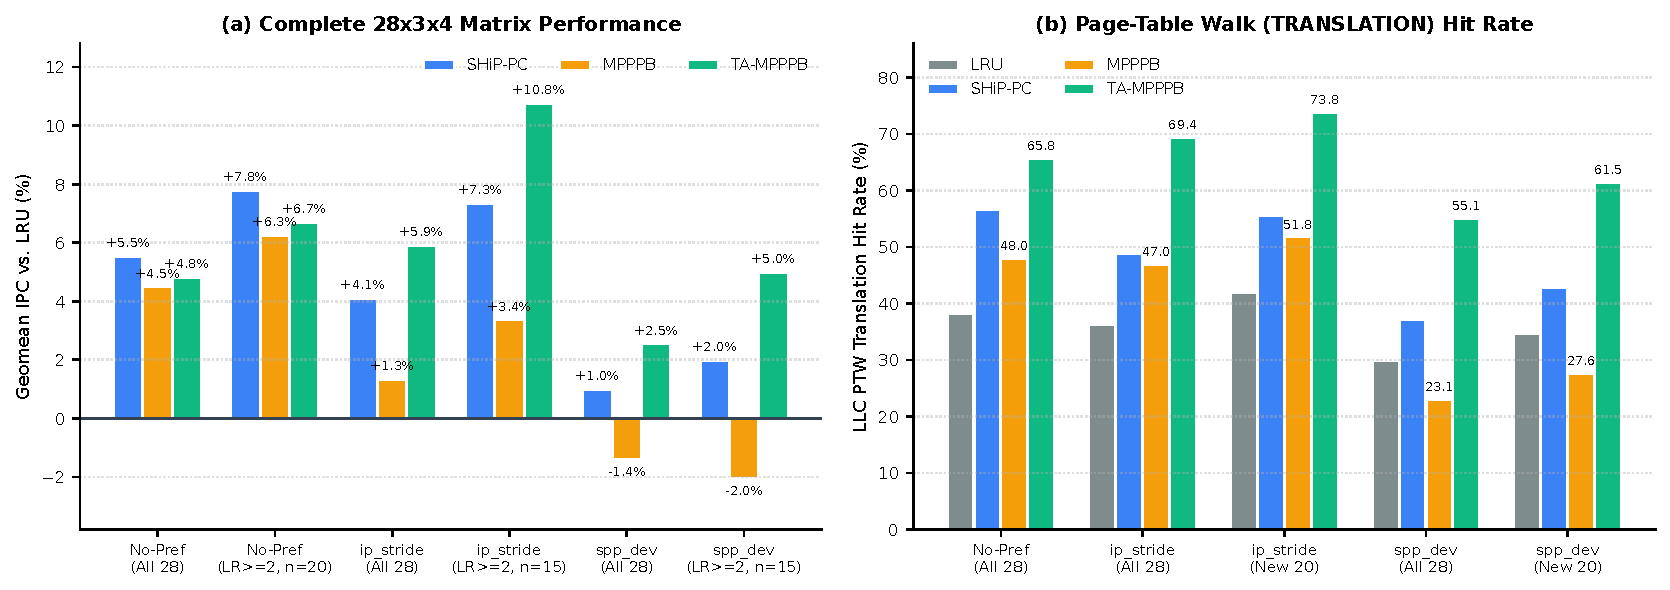
\includegraphics[width=0.96\textwidth]{fig3_matrix_3x28.pdf}
  \caption{28 负载 $\times$ 3 预取体系 $\times$ 4 策略全满贯矩阵汇总（336 场主对比）：(a) 全集与核需求活跃子集（$\mathrm{LR\text{-}MPKI}\ge 2$）相对同组 LRU 的几何平均 IPC 加速比；(b) 全量负载下 \texttt{TRANSLATION} 页表游走请求在 LLC 中的聚合命中率恢复对比。}
  \label{fig:matrix_3x28}
\end{figure*}

\begin{table*}[t]
\centering
\caption{28 负载 $\times$ 3 预取体系 $\times$ 4 策略全矩阵综合性能与指标对比（336 场仿真）}
\label{tab:matrix_summary}
\zihao{6}
\resizebox{\textwidth}{!}{
\begin{tabular}{@{}lcrrrrrrrrrr@{}}
\toprule
\multirow{2}{*}{预取体制与统计子集} & \multirow{2}{*}{$n$} & \multicolumn{3}{c}{相对 LRU Geomean IPC (\%)} & \multicolumn{2}{c}{TA 净优势 (\%)} & \multicolumn{2}{c}{均值 LR-MPKI} & \multicolumn{2}{c}{PTW 命中率 (\%)} & \multirow{2}{*}{W/T/L vs.\,\texttt{MPPPB}} \\
\cmidrule(lr){3-5}\cmidrule(lr){6-7}\cmidrule(lr){8-9}\cmidrule(lr){10-11}
 & & \texttt{SHiP-PC} & \texttt{MPPPB} & \textbf{\texttt{TA-MPPPB}} & vs.\,\texttt{SHiP} & vs.\,\texttt{MPPPB} & \texttt{LRU} & \textbf{\texttt{TA}} & \texttt{MPPPB} & \textbf{\texttt{TA}} & \\
\midrule
No-Pref（全集） & 28 & $+5.54$ & $+4.49$ & $\mathbf{+4.82}$ & $-0.69$ & $+0.32$ & $16.45$ & $13.24$ & $48.04$ & $\mathbf{65.75}$ & $8/17/3$ \\
No-Pref（\texttt{OLD\_8}） & 8 & $+4.30$ & $+4.44$ & $\mathbf{+4.72}$ & $+0.41$ & $+0.28$ & $14.29$ & $12.96$ & $29.99$ & $\mathbf{54.43}$ & $2/6/0$ \\
No-Pref（\texttt{NEW\_20}） & 20 & $+6.05$ & $+4.51$ & $\mathbf{+4.86}$ & $-1.12$ & $+0.33$ & $17.31$ & $13.34$ & $52.79$ & $\mathbf{68.73}$ & $6/11/3$ \\
No-Pref（\texttt{LR-MPKI$\ge$2}） & 20 & $+7.79$ & $+6.26$ & $\mathbf{+6.70}$ & $-1.01$ & $+0.41$ & $22.83$ & $18.34$ & $47.63$ & $\mathbf{65.55}$ & $8/9/3$ \\
\midrule
\texttt{ip\_stride}（全集） & 28 & $+4.10$ & $+1.34$ & $\mathbf{+5.91}$ & $\mathbf{+1.75}$ & $\mathbf{+4.51}$ & $10.84$ & $\mathbf{7.38}$ & $46.98$ & $\mathbf{69.38}$ & $14/13/1$ \\
\texttt{ip\_stride}（\texttt{OLD\_8}） & 8 & $+2.56$ & $+1.66$ & $\mathbf{+3.33}$ & $+0.75$ & $+1.64$ & $9.64$ & $\mathbf{8.68}$ & $27.12$ & $\mathbf{51.28}$ & $4/4/0$ \\
\texttt{ip\_stride}（\texttt{NEW\_20}） & 20 & $+4.72$ & $+1.22$ & $\mathbf{+6.97}$ & $\mathbf{+2.15}$ & $\mathbf{+5.68}$ & $11.33$ & $\mathbf{6.86}$ & $51.82$ & $\mathbf{73.79}$ & $10/9/1$ \\
\texttt{ip\_stride}（\texttt{AllMPKI$\ge$5}） & 20 & $+5.68$ & $+1.83$ & $\mathbf{+8.24}$ & $+2.43$ & $+6.30$ & $15.02$ & $\mathbf{10.18}$ & $46.14$ & $\mathbf{68.91}$ & $13/6/1$ \\
\texttt{ip\_stride}（\texttt{LR-MPKI$\ge$2}） & 15 & $+7.34$ & $+3.36$ & $\mathbf{+10.76}$ & $\mathbf{+3.18}$ & $\mathbf{+7.16}$ & $19.82$ & $\mathbf{13.37}$ & $46.65$ & $\mathbf{69.13}$ & $11/3/1$ \\
\midrule
\texttt{spp\_dev}（全集） & 28 & $+0.99$ & $-1.40$ & $\mathbf{+2.55}$ & $\mathbf{+1.54}$ & $\mathbf{+4.00}$ & $9.20$ & $\mathbf{7.48}$ & $23.07$ & $\mathbf{55.14}$ & $18/9/1$ \\
\texttt{spp\_dev}（\texttt{OLD\_8}） & 8 & $+0.26$ & $-2.19$ & $\mathbf{+1.06}$ & $+0.80$ & $\mathbf{+3.32}$ & $8.44$ & $\mathbf{8.31}$ & $4.50$ & $\mathbf{29.02}$ & $6/2/0$ \\
\texttt{spp\_dev}（\texttt{NEW\_20}） & 20 & $+1.28$ & $-1.08$ & $\mathbf{+3.15}$ & $\mathbf{+1.84}$ & $\mathbf{+4.28}$ & $9.50$ & $\mathbf{7.14}$ & $27.58$ & $\mathbf{61.49}$ & $12/7/1$ \\
\texttt{spp\_dev}（\texttt{AllMPKI$\ge$5}） & 20 & $+1.33$ & $-1.91$ & $\mathbf{+3.55}$ & $+2.19$ & $+5.56$ & $12.71$ & $\mathbf{10.30}$ & $21.84$ & $\mathbf{54.52}$ & $17/2/1$ \\
\texttt{spp\_dev}（\texttt{LR-MPKI$\ge$2}） & 15 & $+1.98$ & $-2.04$ & $\mathbf{+4.99}$ & $\mathbf{+2.95}$ & $\mathbf{+7.18}$ & $16.79$ & $\mathbf{13.57}$ & $21.73$ & $\mathbf{55.07}$ & $\mathbf{15/0/0}$ \\
\bottomrule
\end{tabular}}
\end{table*}

表~\ref{tab:matrix_summary} 客观揭示出三项横跨全预取体制的一致结论：
\begin{enumerate}
  \item \textbf{无预取对照组验证“干净环境等价、混流保护占优”}：在无任何硬件预取干扰时，全 28 负载下 \texttt{MPPPB} 保持 $+4.49\%$，而 \texttt{TA-MPPPB} 小幅超越原版至 $+4.82\%$（胜/平/负 $8/17/3$），并将页表命中率由 $48.04\%$ 抬升至 $65.75\%$。值得实事求是指出的是，在无预取下的 \texttt{dpc3\_6xx} 上 \texttt{SHiP-PC}（$+11.33\%$）主要凭借在极高缺失抖动负载 \texttt{605.mcf\_s}（$\mathrm{LR\text{-}MPKI}=124.36$，SHiP $+82.25\%$ vs. TA $+57.36\%$）和 \texttt{623.xalancbmk\_s}（$+45.67\%$ vs. $+37.55\%$）的极端 RRPV-3 流式截断而短暂领先；但该单特征截断策略一旦遇到现代预取器便迅速失准。
  \item \textbf{开启预取器后的强烈性能反转与 TA-MPPPB 全面领先}：在 \texttt{ip\_stride} 下，全 28 负载中 \texttt{SHiP-PC} 退至 $+4.10\%$，原版 \texttt{MPPPB} 坠至 $+1.34\%$，而 \texttt{TA-MPPPB} 跃升至 \textbf{+5.91\%}（超越 SHiP-PC $+1.75\%$、超越 MPPPB $+4.51\%$），将核阻塞需求 \texttt{LR-MPKI} 由 $10.84$ 大幅压降至 \textbf{7.38}（降幅 \textbf{$-31.9\%$}），活跃子集 \texttt{LR-MPKI$\ge$2} 加速高达 \textbf{+10.76\%}。
  \item \textbf{\texttt{spp\_dev} 高强度预取洪峰下的鲁棒胜出}：当 L2 预取器切换为 \texttt{spp\_dev} 时，全 28 负载下 LLC 总预取请求量从 $5{,}157$ 万次暴增至 $2.50$ 亿次。在此冲击下，原版 \texttt{MPPPB} 全面崩溃至 \textbf{-1.40\%}（页表命中率跌破 LRU 的 $29.99\%$，仅余 \textbf{23.07\%}），\texttt{SHiP-PC} 亦跌破 $1\%$（$+0.99\%$）；而 \texttt{TA-MPPPB} 依然斩获 \textbf{+2.55\%}（vs. SHiP-PC $+1.54\%$、vs. MPPPB $+4.00\%$），在 15 条高需求压力负载上对原版 MPPPB 达成 \textbf{15/0/0（100\% 全胜）}。
\end{enumerate}

\subsection{分数据集（Suite）与代表性负载对比}

表~\ref{tab:suites} 按全部 5 个独立数据集展开跨预取体制总结，图~\ref{fig:highlights} 展示了涵盖 5 个 Suite 全部代表性场景（同时包含显式大幅胜出、负向退化挽救、读写权衡以及中性/微幅回退边界）的 14 条代表性负载逐项表现。

\begin{table}[t]
\centering
\caption{全 5 大数据集（28 负载）在双预取器下的分 Suite Geomean 对比}
\label{tab:suites}
\zihao{6}
\resizebox{\columnwidth}{!}{
\begin{tabular}{@{}lrrrrr@{}}
\toprule
\multirow{2}{*}{预取器与 Suite（$n$）} & \multicolumn{3}{c}{Geomean IPC vs.\,LRU (\%)} & \multicolumn{2}{c}{PTW 命中率 (\%)} \\
\cmidrule(lr){2-4}\cmidrule(lr){5-6}
 & \texttt{SHiP-PC} & \texttt{MPPPB} & \textbf{\texttt{TA-MPPPB}} & \texttt{MPPPB} & \textbf{\texttt{TA}} \\
\midrule
\texttt{ip\_stride}: \texttt{spec06\_4xx} (8) & $+2.56$ & $+1.66$ & $\mathbf{+3.33}$ & $27.12$ & $\mathbf{51.28}$ \\
\texttt{ip\_stride}: \texttt{dpc3\_6xx} (10) & $+8.39$ & $+2.29$ & $\mathbf{+12.68}$ & $48.83$ & $\mathbf{82.04}$ \\
\texttt{ip\_stride}: \texttt{zenodo\_gap\_xs} (4) & $+2.32$ & $+1.13$ & $\mathbf{+2.38}$ & $53.32$ & $\mathbf{67.82}$ \\
\texttt{ip\_stride}: \texttt{zenodo\_cvp1} (3) & $+1.01$ & $-0.67$ & $\mathbf{+2.10}$ & $55.65$ & $\mathbf{77.66}$ \\
\texttt{ip\_stride}: \texttt{zenodo\_qualcomm} (3) & $-0.18$ & $-0.31$ & $-0.13$ & $89.01$ & $90.74$ \\
\midrule
\texttt{spp\_dev}: \texttt{spec06\_4xx} (8) & $+0.26$ & $-2.19$ & $\mathbf{+1.06}$ & $4.50$ & $\mathbf{29.02}$ \\
\texttt{spp\_dev}: \texttt{dpc3\_6xx} (10) & $+2.04$ & $-0.96$ & $\mathbf{+4.80}$ & $35.22$ & $\mathbf{69.97}$ \\
\texttt{spp\_dev}: \texttt{zenodo\_gap\_xs} (4) & $+0.88$ & $-1.87$ & $\mathbf{+1.43}$ & $20.95$ & $\mathbf{54.98}$ \\
\texttt{spp\_dev}: \texttt{zenodo\_cvp1} (3) & $+0.77$ & $-1.19$ & $\mathbf{+3.36}$ & $43.07$ & $\mathbf{70.28}$ \\
\texttt{spp\_dev}: \texttt{zenodo\_qualcomm} (3) & $-0.18$ & $-0.33$ & $-0.17$ & $84.44$ & $84.45$ \\
\bottomrule
\end{tabular}}
\end{table}

\begin{figure*}[t]
  \centering
  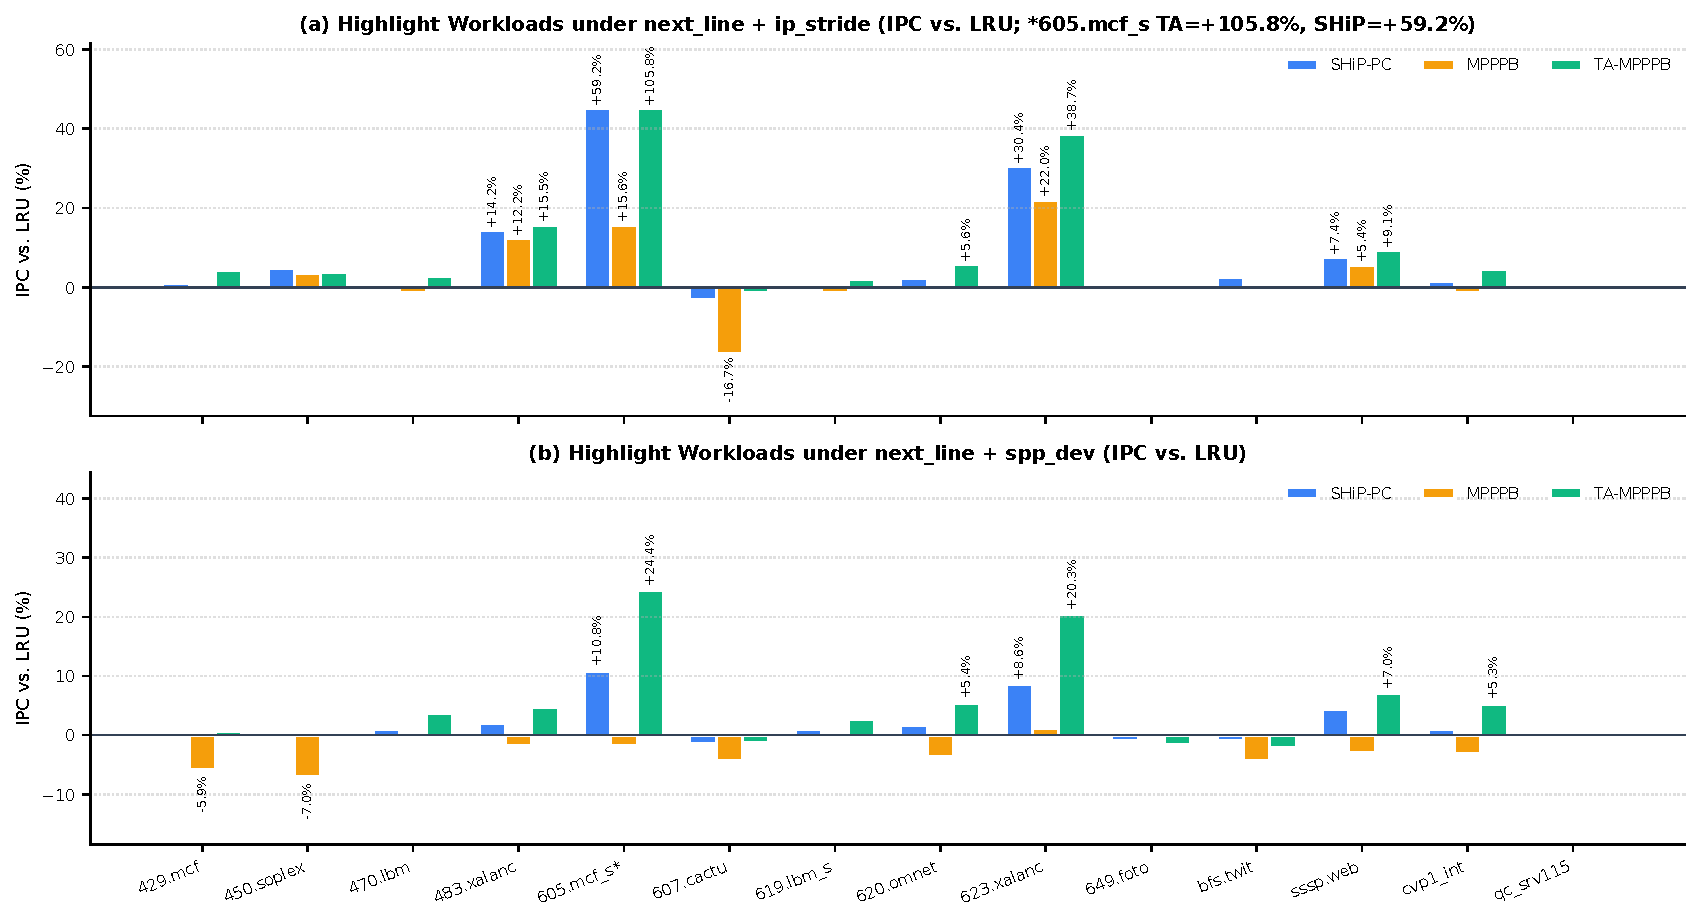
\includegraphics[width=0.96\textwidth]{fig4_highlights.pdf}
  \caption{跨 5 大基准集代表性活跃工作负载逐项 IPC 加速比对比（兼顾高增益、崩塌挽回与负向/中性边界）：(a) \texttt{next\_line}+\texttt{ip\_stride}；(b) \texttt{next\_line}+\texttt{spp\_dev}。}
  \label{fig:highlights}
\end{figure*}

可以观察到，TA-MPPPB 在全部 4 个 LLC 压力活跃的独立数据集中均同时稳居第一（\texttt{zenodo\_qualcomm} 因 2 MiB LLC 下 $\mathrm{LR\text{-}MPKI}<0.55$ 而预期呈中性持平，差值 $<0.3\%$）：
\begin{itemize}
  \item \textbf{链式指针与高页表压力负载}：在 \texttt{605.\allowbreak mcf\_s} 与 \texttt{623.\allowbreak xalancbmk\_s} 上，\texttt{ip\_stride} 下 TA-MPPPB 分别提速 \textbf{+105.83\%}（SHiP $+59.18\%$、MPPPB $+15.59\%$）与 \textbf{+38.66\%}（页表命中率由 $3.71\%$ 跃升至 \textbf{92.72\%}）；\texttt{spp\_dev} 下同样大幅领先（\textbf{+24.44\%} 与 \textbf{+20.34\%}）。
  \item \textbf{大图计算与整数计算}：在 \texttt{sssp.\allowbreak web} 上分别获得 \textbf{+9.15\%}（\texttt{ip\_stride}）与 \textbf{+7.01\%}（\texttt{spp\_dev}），超越原版 MPPPB $+3.51\%$ 与 $+10.30\%$；在 \texttt{cvp1\_\allowbreak compute\_\allowbreak int\_38} 上由原版 MPPPB 负向退化（$-1.31\% / -3.13\%$）强势反转为 \textbf{+4.37\%} 与 \textbf{+5.25\%}。
  \item \textbf{预取保护与规律负载挽回}：在规律步长模拟 \texttt{607.\allowbreak cactuBSSN\_s} 上，原版 MPPPB 因盲目旁路 $98.1$ 万次有用预取而在 \texttt{ip\_stride} 暴跌 $-16.67\%$；TA-MPPPB 借助 \texttt{pfsel\_} 将有用预取保护于 $\mathrm{PLRU}=8$，拉回至 $-1.40\%$（相对原版 MPPPB 追回 \textbf{+18.32\%}，且在 \texttt{ip\_stride} / \texttt{spp\_dev} 均优于 SHiP-PC）。
\end{itemize}

\subsection{集合决斗自适应分化与写回—需求权衡分析}

汇总 \texttt{G1}（SPEC06+\texttt{spp\_dev}）、\texttt{G2}（New-20+\texttt{ip\_stride}）、\texttt{G3}（New-20+\texttt{spp\_dev}）的运行探针与全 28 负载流量统计（表~\ref{tab:probe_stats}）以及决斗计数器分化象限（图~\ref{fig:mechanism}），揭示了 TA-MPPPB 实现鲁棒性的内在闭环：

\begin{table}[t]
\centering
\caption{跨体制旁路计数（\texttt{g\_probe}）与全 28 负载 ROI 流量命中/缺失聚合统计}
\label{tab:probe_stats}
\zihao{6}
\resizebox{\columnwidth}{!}{
\begin{tabular}{@{}llrrr@{}}
\toprule
统计范畴 & 策略 & 旁路 (\texttt{dem / pref / tr}) & \texttt{PREF} 命中 & \texttt{WRITE} 缺失 \\
\midrule
G1 (Old-8, \texttt{spp}) & \texttt{MPPPB} & $14.11\text{M}$ ($6.54\text{M}/7.09\text{M}/0.48\text{M}$) & $38.31\%$ & $7.55\%$ \\
G1 (Old-8, \texttt{spp}) & \textbf{\texttt{TA-MPPPB}} & $5.68\text{M}$ ($5.68\text{M}/\mathbf{0}/\mathbf{0}$) & $\mathbf{41.87\%}$ & $\mathbf{45.38\%}$ \\
\midrule
G2 (New-20, \texttt{ip}) & \texttt{MPPPB} & $63.33\text{M}$ ($24.04\text{M}/38.35\text{M}/0.94\text{M}$) & $12.35\%$ & $21.00\%$ \\
G2 (New-20, \texttt{ip}) & \textbf{\texttt{TA-MPPPB}} & $9.20\text{M}$ ($9.20\text{M}/\mathbf{0}/\mathbf{0}$) & $\mathbf{19.89\%}$ & $\mathbf{66.68\%}$ \\
\midrule
G3 (New-20, \texttt{spp}) & \texttt{MPPPB} & $39.26\text{M}$ ($18.75\text{M}/19.16\text{M}/1.35\text{M}$) & $48.82\%$ & $6.31\%$ \\
G3 (New-20, \texttt{spp}) & \textbf{\texttt{TA-MPPPB}} & $8.01\text{M}$ ($8.01\text{M}/\mathbf{0}/\mathbf{0}$) & $\mathbf{51.64\%}$ & $\mathbf{61.08\%}$ \\
\midrule
\multirow{3}{*}{All-28 \texttt{ip\_stride}} & \texttt{LRU} & — & $7.58\%$ & $0.11\%$ \\
 & \texttt{MPPPB} & — & $13.35\%$ & $15.38\%$ \\
 & \textbf{\texttt{TA-MPPPB}} & — & $\mathbf{18.73\%}$ & $\mathbf{54.01\%}$ \\
\midrule
\multirow{3}{*}{All-28 \texttt{spp\_dev}} & \texttt{LRU} & — & $42.95\%$ & $0.22\%$ \\
 & \texttt{MPPPB} & — & $46.74\%$ & $6.99\%$ \\
 & \textbf{\texttt{TA-MPPPB}} & — & $\mathbf{49.64\%}$ & $\mathbf{52.48\%}$ \\
\bottomrule
\end{tabular}}
\end{table}

\begin{figure*}[t]
  \centering
  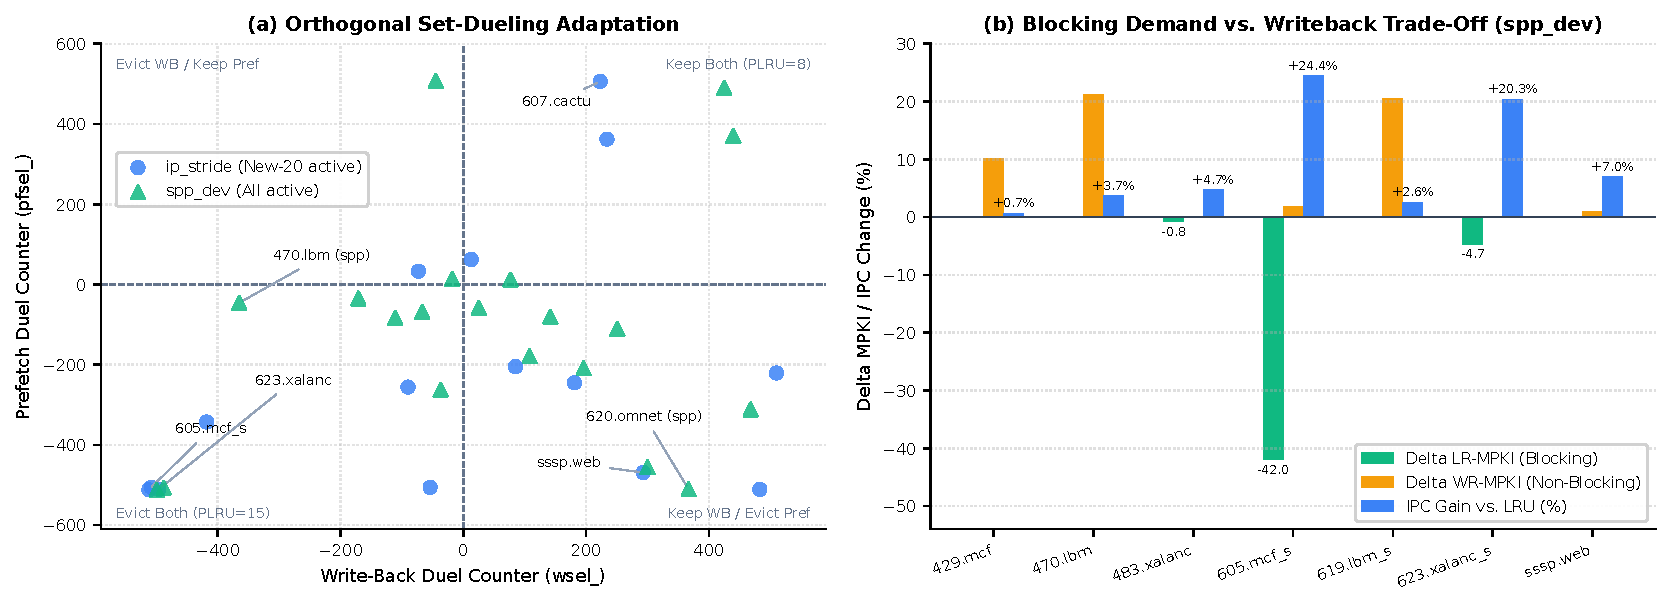
\includegraphics[width=0.96\textwidth]{fig5_mechanism.pdf}
  \caption{TA-MPPPB 内部自适应决斗分化与流量权衡：(a) 活跃负载下 \texttt{wsel\_} 与 \texttt{pfsel\_} 饱和分布呈现清晰的四象限自适应；(b) 阻塞型核需求 \texttt{LR-MPKI} 下降与非阻塞后台 \texttt{WR-MPKI} 提升的性能权衡机理。}
  \label{fig:mechanism}
\end{figure*}

\begin{enumerate}
  \item \textbf{扭转“旁路预取页表、却蓄养死写回”的错配}：原版 MPPPB 在 \texttt{spp\_dev} 28 负载下允许高达 $93.01\%$ 的后台 \texttt{WRITE} 命中驻留（缺失率仅 $6.99\%$），却旁路了 $2{,}624$ 万次预取与 $183.7$ 万次页表。TA-MPPPB 彻底清零预取/页表旁路并以 \texttt{wsel\_} 适度卸载流式脏写回（\texttt{WRITE} 缺失率升至 $52.48\%\sim 54.01\%$），反使 \texttt{PREFETCH} 在 LLC 中的命中率全面超越原版（All-28 \texttt{ip\_stride} $13.35\%\to 18.73\%$，\texttt{spp\_dev} $46.74\%\to 49.64\%$）。
  \item \textbf{四象限精确自适应}：如图~\ref{fig:mechanism}(a) 所示，高污染抖动负载（\texttt{605.mcf\_s}、\texttt{623.xalancbmk\_s}）上 \texttt{wsel\_} 与 \texttt{pfsel\_} 双双收敛至左下极值（$-496\sim -512$），将其迅速驱离核心工作集；高精度预取负载（\texttt{607.cactuBSSN\_s}）跃升至右上象限（\texttt{wsel=+223}, \texttt{pfsel=+506}）；写重用较高但预取污染较大的 \texttt{620.omnetpp\_s} 与 \texttt{sssp.web} 自动落入右下象限（保留写回、淘汰预取）。
  \item \textbf{非阻塞写回与阻塞需求之间的客观交换}：如图~\ref{fig:mechanism}(b) 所示，在流式网格 \texttt{470.lbm} 与 \texttt{619.lbm\_s}（\texttt{spp\_dev}）上，\texttt{wsel\_}（$-365$ 与 $-37$）将脏写回推至 $\mathrm{PLRU}=15$，使非阻塞 \texttt{WR-MPKI} 由 $\sim 0.00$ 升至 $21.16$ 与 $20.49$，换回 \texttt{470.lbm} 页表命中率从 $0\%$ 恢复至 $10.45\%$ 并实现 \textbf{+3.69\%} 与 \textbf{+2.59\%} IPC 加速。
\end{enumerate}

%======================================================================
\section{全 28 负载双预取器消融、MSHR 实证与边界讨论}
%======================================================================

\subsection{全 28 负载 $\times$ 双预取器留一法（LOO）与动态决斗消融}

为彻底检验 TA-MPPPB 每一处架构组件的真实必要性，我们在最终定型代码上新增正交开关 \texttt{MPPPB\_LOO}，针对全 28 负载 $\times$ 双预取器（\texttt{ip\_stride} 与 \texttt{spp\_dev}）分别执行四大组件的精确单模块剔除（Leave-One-Out），并额外验证将固定中游页表保护替换为动态页表集合决斗（\texttt{+PTW Set-Duel}：\texttt{MPPPB\_TRANS\_DUEL=1}，在 $\mathrm{PLRU}=8$ 与 $15$ 间由需求缺失决斗），总计完成 \textbf{280 场消融仿真}。汇总结果列于表~\ref{tab:loo_full} 与图~\ref{fig:loo_ablation}。

\begin{table*}[t]
\centering
\caption{全 28 负载 $\times$ 双预取器正交留一法（LOO）与动态页表决斗消融汇总（280 场仿真，基准为完整 TA-MPPPB）}
\label{tab:loo_full}
\zihao{6}
\resizebox{\textwidth}{!}{
\begin{tabular}{@{}lrrrrrrrrrr@{}}
\toprule
\multirow{2}{*}{消融变体（相对完整 TA）} & \multicolumn{5}{c}{\texttt{next\_line} + \texttt{ip\_stride}} & \multicolumn{5}{c}{\texttt{next\_line} + \texttt{spp\_dev}} \\
\cmidrule(lr){2-6}\cmidrule(lr){7-11}
 & All-28 & LR$\ge$2 & 最差单条 & PTW 命中率 & W/T/L(All) & All-28 & LR$\ge$2 & 最差单条 & PTW 命中率 & W/T/L(All) \\
\midrule
完整 \texttt{TA-MPPPB}（基准） & $0.00\%$ & $0.00\%$ & — & $69.38\%$ & — & $0.00\%$ & $0.00\%$ & — & $55.14\%$ & — \\
\texttt{w/o Zero-PC Shield} & $+0.14\%$ & $+0.28\%$ & $-0.42\%$ & $68.82\%$ & $1/27/0$ & $-0.02\%$ & $-0.07\%$ & $-0.60\%$ & $54.91\%$ & $0/27/1$ \\
\texttt{w/o PTW Protection} & $-0.28\%$ & $-0.40\%$ & $-3.16\%$ & $57.11\%$ & $1/20/7$ & $-0.38\%$ & $-0.70\%$ & $-3.15\%$ & $42.87\%$ & $0/22/6$ \\
\texttt{w/o Write Arbitration} & $-0.56\%$ & $-0.97\%$ & $-4.89\%$ & $67.67\%$ & $1/20/7$ & $-0.49\%$ & $-0.91\%$ & $-3.86\%$ & $54.07\%$ & $3/18/7$ \\
\texttt{w/o Prefetch Arbitration} & $\mathbf{-1.15\%}$ & $\mathbf{-1.51\%}$ & $\mathbf{-7.42\%}$ & $68.45\%$ & $3/13/12$ & $\mathbf{-2.12\%}$ & $\mathbf{-3.88\%}$ & $\mathbf{-15.85\%}$ & $37.81\%$ & $2/16/10$ \\
\texttt{+PTW Set-Duel}（对照） & $\mathbf{-1.72\%}$ & $\mathbf{-2.91\%}$ & $\mathbf{-13.60\%}$ & $\mathbf{15.78\%}$ & $2/19/7$ & $\mathbf{-1.61\%}$ & $\mathbf{-2.75\%}$ & $\mathbf{-12.05\%}$ & $\mathbf{12.88\%}$ & $0/21/7$ \\
\bottomrule
\end{tabular}}
\end{table*}

\begin{figure*}[t]
  \centering
  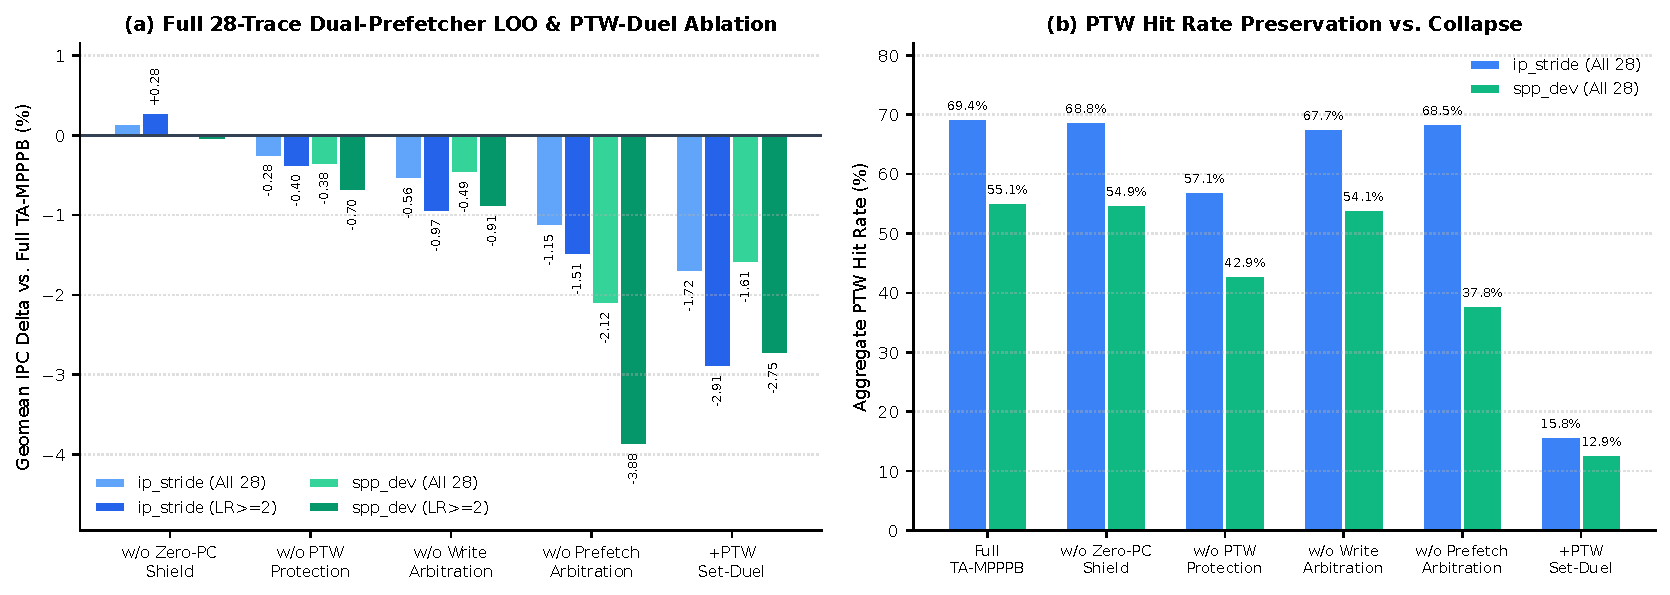
\includegraphics[width=0.96\textwidth]{fig6_loo_ablation.pdf}
  \caption{全 28 负载 $\times$ 双预取器（\texttt{ip\_stride} 与 \texttt{spp\_dev}）留一法消融及动态页表决斗失效实证：(a) 各模块移除或替换相对完整 TA-MPPPB 的几何平均 IPC 变化；(b) 全 28 负载 \texttt{TRANSLATION} 命中率保持与崩溃对比。}
  \label{fig:loo_ablation}
\end{figure*}

全量 28 负载双预取器 LOO 消融揭示了四项极具说服力的定量证据：
\begin{enumerate}
  \item \textbf{预取仲裁（Prefetch Arbitration）是首要性能支柱}：移除该模块后，全 28 负载在 \texttt{ip\_stride} 与 \texttt{spp\_dev} 下几何平均性能分别骤降 \mbox{\textbf{$-1.15\%$}}（活跃子集 $-1.51\%$，最差 \texttt{607.cactuBSSN\_s} 暴跌 $-7.42\%$）与 \mbox{\textbf{$-2.12\%$}}（活跃子集高达 \mbox{\textbf{$-3.88\%$}}，\texttt{605.mcf\_s} 暴跌 \mbox{\textbf{$-15.85\%$}}、\texttt{623.xalancbmk\_s} 暴跌 \mbox{\textbf{$-14.38\%$}}），同时 \texttt{spp\_dev} 下页表命中率由 $55.14\%$ 被重创至 $37.81\%$。
  \item \textbf{写回仲裁（Write Arbitration）稳定贡献跨预取正收益}：剔除 \texttt{wsel\_} 与写回采样隔离后，两预取体制全集均稳步受损 $-0.56\%$ 与 $-0.49\%$（活跃子集各约 $-0.97\%$ 与 $-0.91\%$），在 \texttt{605.mcf\_s}（$-4.90\%$）、\texttt{429.mcf}（$-3.50\%$）、\texttt{470.lbm}（$-3.38\%$）与 \texttt{cvp1\_compute\_fp\_8}（$-3.86\%$）上均出现显著回退。
  \item \textbf{PTW 固定中游保护不可替代，且动态 PTW 决斗（\texttt{+PTW Set-Duel}）全盘溃败}：移除 PTW 保护使两个预取器下的页表命中率均立即坠落 \textbf{12.3 个百分点}（$69.38\%\to 57.11\%$，$55.14\%\to 42.87\%$），在 \texttt{spp\_dev} 上导致 $0/22/6$ 无一胜出（\texttt{sssp.web} $-3.16\%$、\texttt{623.xalancbmk\_s} $-2.08\%$）。更为关键的是，全 28 负载检验推翻了局部旧负载上的保守认知：若将固定 $\mathrm{PLRU}=8$ 替换为动态需求加权决斗 \texttt{+PTW Set-Duel}，由于低频页表缺失在领跑组中被高频 \texttt{LOAD/RFO} 噪声淹没，\texttt{tsel\_} 普遍漂向负数并把页表锁定在 $\mathrm{PLRU}=15$ 极速淘汰位，致使全 28 负载 PTW 命中率从 $69.38\% / 55.14\%$ \textbf{断崖式崩塌至 $15.78\% / 12.88\%$}，整体性能暴跌 \mbox{\textbf{$-1.72\%$}}\,/\,\mbox{\textbf{$-1.61\%$}}（\texttt{620.omnetpp\_s} $-13.60\%$、\texttt{sssp.web} $-13.45\%$、\texttt{cvp1\_int} $-11.82\%$）。这以全量实证严格解释了为何 TA-MPPPB 必须对低频页表采用确定性中游保护，而仅对高频写回/预取采用集合决斗。
  \item \textbf{Zero-PC 屏蔽的下游结构冗余裕量解析}：单独撤去 \texttt{Zero-PC Shield} 时，全 28 负载在 \texttt{spp\_dev} 下呈轻微负向（$-0.02\%$，\texttt{sssp.web} $-0.60\%$，$0/27/1$），而在 \texttt{ip\_stride} 下有 27/28 条持平（$1/27/0$），仅 \texttt{605.mcf\_s} 意外偏高 $+4.81\%$（统计核查显示其 0 号权重泄漏微调了 \texttt{LOAD} 旁路分数，以 $+43.1$ 万次预取缺失换取 $-48.5$ 万次需求加载缺失）。其微幅边际变化的原因十分清晰：在完整 TA-MPPPB 中，下游的预取隔离、写回隔离与 PTW 保护三道闸门已经提前将绝大部分 $\mathrm{ip}=0$ 访问挡在了采样器与放置评分之外，因此前端 Zero-PC 屏蔽主要作为正交“纵深防御”兜底阻断零值进入 \texttt{pc\_ring}（前向归因第 3.3 节已证实在未加下游隔离的基线 MPPPB 上清理 Zero-PC 立即带来 $+0.22\%\sim +0.24\%$ 收益）。
\end{enumerate}

\subsection{\texorpdfstring{\texttt{effective\_ip} 页号哈希与 MSHR 合并耦合实证}{effective\_ip 页号哈希与 MSHR 合并耦合实证}}

在架构探索中，我们曾设计在 \texttt{effective\_ip()} 中为 $\mathrm{ip}=0$ 的 \texttt{PREFETCH} 请求构造基于 4 KiB 页号的伪 PC（$\texttt{0x9e3779b9ULL}\oplus (\mathrm{block}\gg 6)$）以缓解哈希冲突。而在 TA-MPPPB 定型后，因 \texttt{PREFETCH} 已全面切入 \texttt{pfsel\_} 决斗与采样器隔离路径，该页号哈希在定型版本中处于静默未激活状态。

为严密核实这一静默路径是否隐藏微架构差异，我们建立独立分支 \texttt{exp/\allowbreak activate-\allowbreak effective-\allowbreak ip-\allowbreak hash}，强制激活该页号哈希并对高预取负载 \texttt{649.\allowbreak fotonik3d\_s} 与 \texttt{623.\allowbreak xalancbmk\_s} 在双预取器下实测对比（表~\ref{tab:effip_mshr}）。结果显示：当无核读撞上在途预取（\texttt{LOAD miss\_merge=0}，即 \texttt{ip\_stride} 下的 \texttt{649.\allowbreak fotonik3d\_s}）时，激活页号哈希后的执行周期与主干严格一致（同为 $207{,}672{,}023$ 周期，差异精确为 $0$）；仅当存在大量需求读与在途预取 MSHR 合并（\texttt{fill\_type::merge}，如 \texttt{spp\_dev} 下的 \texttt{623.\allowbreak xalancbmk\_s} 出现 5.7\,万次合并）时，由于合并后的填充复用 \texttt{in\_flight\_} 队列中原先由在途 \texttt{PREFETCH} 压入的旧评分来指导后续需求行决策，才经 1.5\,亿条指令形成 $<0.23\%$（$-0.0008\%\sim +0.2225\%$）的时序微扰，对宏观排序结论毫无影响，却精准指出未来在 MSHR 类型升级时覆写最新 \texttt{LOAD} 评分的精细优化点。

\begin{table}[t]
\centering
\caption{分支 \texttt{exp/activate-effective-ip-hash} 激活页号哈希实测与 MSHR 合并统计}
\label{tab:effip_mshr}
\zihao{6}
\resizebox{\columnwidth}{!}{
\begin{tabular}{@{}llrrr@{}}
\toprule
预取与负载 & 主干周期 & 激活页号哈希周期 & IPC 变化 & \texttt{LOAD miss\_merge}（主干/分支） \\
\midrule
\texttt{ip\_stride} / \texttt{649.fotonik3d\_s} & $207{,}672{,}023$ & $207{,}672{,}023$ & $+0.0000\%$ & $0\ /\ 0$ \\
\texttt{ip\_stride} / \texttt{623.xalancbmk\_s} & $320{,}754{,}531$ & $320{,}042{,}575$ & $+0.2225\%$ & $1\ /\ 1$ \\
\texttt{spp\_dev} / \texttt{649.fotonik3d\_s} & $88{,}239{,}335$ & $88{,}240{,}080$ & $-0.0008\%$ & $6{,}342\ /\ 6{,}359$ \\
\texttt{spp\_dev} / \texttt{623.xalancbmk\_s} & $343{,}111{,}133$ & $342{,}625{,}577$ & $+0.1417\%$ & $51{,}803\ /\ 57{,}055$ \\
\bottomrule
\end{tabular}}
\end{table}

\subsection{局限性边界分析与未来工作}

本着科学客观原则，我们对全 28 负载评测中的极少数回退个例及体系结构局限作如下界定：
\begin{enumerate}
  \item \textbf{极低需求缺失率下的预取决斗盲区}：在 \texttt{spp\_dev} 下的 \texttt{649.\allowbreak fotonik3d\_s} 上，TA-MPPPB 相对 LRU 出现 $-1.58\%$ 回退（相对 SHiP-PC $-0.68\%$）。主干全量日志显示其核心阻塞 \texttt{LR-MPKI} 低至 \textbf{0.20}，而 \texttt{Dem-MPKI} 高达 \textbf{71.92}（TA 下 $70.71$）。极端稀疏的需求监督样本使 \texttt{pfsel\_} 轻微偏冷（$-59$），未来可在 \texttt{LR-MPKI} 低于阈值时引入轻量化预取效用校正项。
  \item \textbf{极高规律与极度随机图遍历极限}：在 \texttt{607.\allowbreak cactuBSSN\_s}（\mbox{$-1.40\%$}\,/\,\mbox{$-1.28\%$}，较原版 MPPPB 大幅挽回 $+18.32\%$）与 \texttt{bfs.\allowbreak twitter-10B}（\texttt{spp\_dev} 下 $-2.08\%$，仍胜原版 MPPPB $+2.25\%$）上，高覆盖常规预测与无规则大图散射逼近局部信息论上限。
  \item \textbf{单核假设与多核共享总线延伸}：本文聚焦单核高覆盖预取验证；若向未来多核共享 LLC 扩展，剧增的非阻塞写回与主存带宽竞争将不再免费，后续可基于核间写队列压力和 \texttt{pfsel\_} 深度负值（如 $\texttt{pfsel\_}<-256$）条件恢复垃圾预取旁路，并彻底为未命中采样器的残留写回行标注 \texttt{zero\_pc} 跳过标志以消除任何反向训练污染。
\end{enumerate}

%======================================================================
\section{结\quad 论}
%======================================================================

本文在完整五级虚存与多级硬件预取 ChampSim 平台上严格复现了 Static MDPP 底座的 MPPPB 算法，并通过跨 5 大基准域 28 条负载与 3 种预取体系的对比实验，首次完整揭示了其在预取器激活后由 $\mathrm{ip}=0$ 异构流量耦合导致的系统性“能力反转”。针对该核心缺陷，本文提出零额外 SRAM 阵列、仅增 20 bits 全局寄存器的 \textbf{TA-MPPPB} 方案，将 Zero-PC 特征隔离、\texttt{TRANSLATION} 零旁路中游保护（$\mathrm{PLRU}=8$）、双模写回采样与需求缺失监督的正交双路集合决斗融为一体。336 场主对比实验与 280 场全负载双预取器留一法消融一致验证：TA-MPPPB 在冻结零调参前提下全面超越 LRU、SHiP-PC 与原版 MPPPB，在 \texttt{ip\_stride} 与 \texttt{spp\_dev} 下全 28 负载加速 $+5.91\%$ 与 $+2.55\%$（活跃负载 $+10.76\%$ 与 $+4.99\%$）、页表命中率抬升至 $69.38\%$ 与 $55.14\%$，同时澄清了固定中游 PTW 保护相对动态决斗的压倒性稳定性优势及 MSHR 合并微扰边界。

\vspace{4pt}
{\noindent\zihao{4}\heiti 致\quad 谢}\quad
{\zihao{5}\songti 感谢开源现代模拟器 ChampSim 社区及 DPC-3、Zenodo 等公开基准轨迹维护者提供可复现的微架构实验基础设施。}

\vspace{2pt}
\bibliographystyle{gbt7714-numerical}
\bibliography{ta_mpppb_refs}

%======================================================================
\vspace{3pt}
\noindent{\zihao{4}\bfseries Background}
\vspace{1pt}

{\noindent\zihao{5-}
Last-level cache (LLC) replacement mitigates the memory wall in out-of-order processors. While perceptron predictors like MPPPB (Static MDPP) perform strongly without prefetching, modern multi-level prefetchers inject zero-PC ($\mathrm{ip}=0$) \texttt{TRANSLATION}, \texttt{WRITE}, and \texttt{PREFETCH} requests into the LLC, triggering Bucket-0 aliasing, history-ring flushing, and false translation bypasses that invert MPPPB below LRU under \texttt{spp\_dev}.

Without altering cross-level buses or enlarging SRAM arrays beyond 32~KiB, TA-MPPPB adds only 20~bits via Zero-PC shielding, non-bypass mid-tree protection ($\mathrm{PLRU}=8$) for \texttt{TRANSLATION}, dual-mode writeback sampling, and demand-miss-weighted orthogonal set dueling (\texttt{wsel\_}, \texttt{pfsel\_}). Evaluated across a complete 28-workload $\times$ 3-regime $\times$ 4-policy matrix and 280 dual-prefetcher LOO ablations (616 runs total), TA-MPPPB outperforms LRU, SHiP-PC, and MPPPB while elevating translation hit rates to $69.38\%$ (\texttt{ip\_stride}) and $55.14\%$ (\texttt{spp\_dev}).}

\end{document}
